

\section{Results}\label{sec:results}
We ran multiple experiments for each optimizer. This Section will  give an overview of the achieved results. Each subsection will give an explanation over the achieved result with a specific optimizer.

\subsubsection{SGD}
The first challenge for each optimizer was to find a correct learning rate. As SGD is the optimizer used in Gensim \cite{gensim} we first tried the same learning rate as the default value in Gensim \cite{gensim}, i.e 0.01,  and then performed a random search to find a better one. As expected a bell curve shape resulted, a learning rate that is too high leads to diversion and a learning rate that is too low leads to a training time that is too slow. The best value that we found for the learning rate is $0.0075$. With this setting SGD converged in 11 epochs. The second experiment was to add input shuffling.
As seen in Figure \ref{fig:results_sgd}, for almost every learning rate the convergence time decreased. Our model, with the best setting, now converges in only 7 epochs. Another interesting fact to point out from Figure \ref{fig:results_sgd} is that with input shuffling we achieved better results with higher learning rates. As for learning rates of $0.01$ and $0.025$ we did converge in 11 epochs with input shuffling but did not converge in 20 epochs without it.

\begin{figure}[h]
\centering
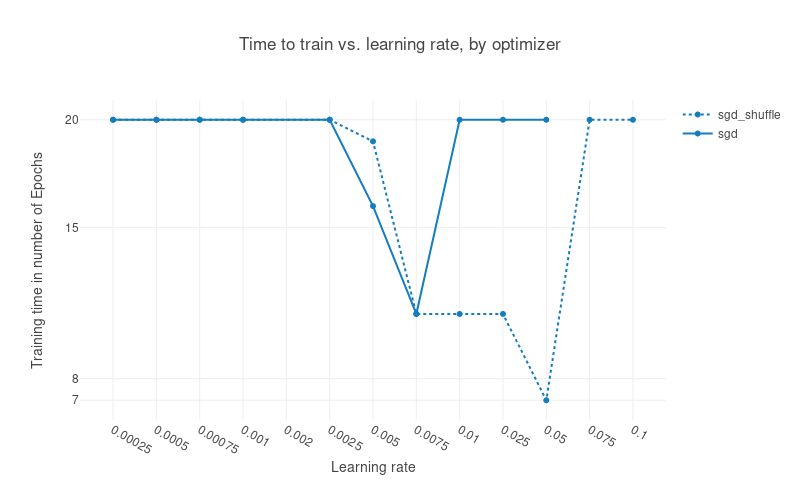
\includegraphics[scale=0.3]{images/results_sgd_shuffle}
\caption{Training time Stochastic Gradient Descent with input Shuffling}
\label{fig:results_sgd}
\end{figure}
\subsubsection{Momentum and Nesterov}
Momentum and NAG \cite{nag} both have an additional hyperparameter $\gamma$, that, defines the percentage of the previous gradient that will be added to the current gradients. We set $\gamma = 0.9$ as this is a typical value and did not alter it during our experiments. Momentum and Nesterov alone respectively only slightly decrease or increase the convergence time. Momentum optimally converges in 9 epochs and Nesterov in 13. If we combine these optimizers with input shuffling, interestingly the same phenomena as with plain SGD appear. The convergence time gets better, 8 epochs for Momentum and 3 epochs for NAG. The phenomena that a higher learning rat yields better results also happens with both of the optimizers. As Momentum does not converge in 20 epochs with a learning rate of 0.002 but does in 8 with input shuffling.
\begin{figure}[h]
\centering

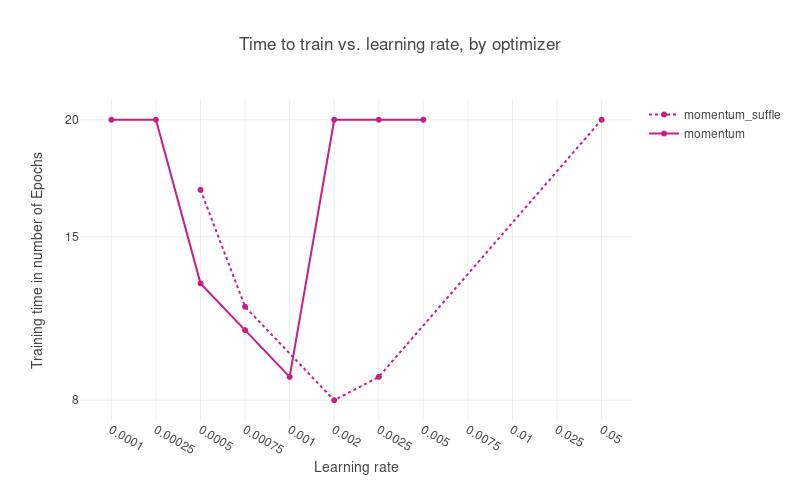
\includegraphics[scale=0.3]{images/results_mom_shuffle}
\caption{Training time Momentum with input Shuffling}
\label{fig:results_mom}
\end{figure}

\begin{figure}[h]
\centering
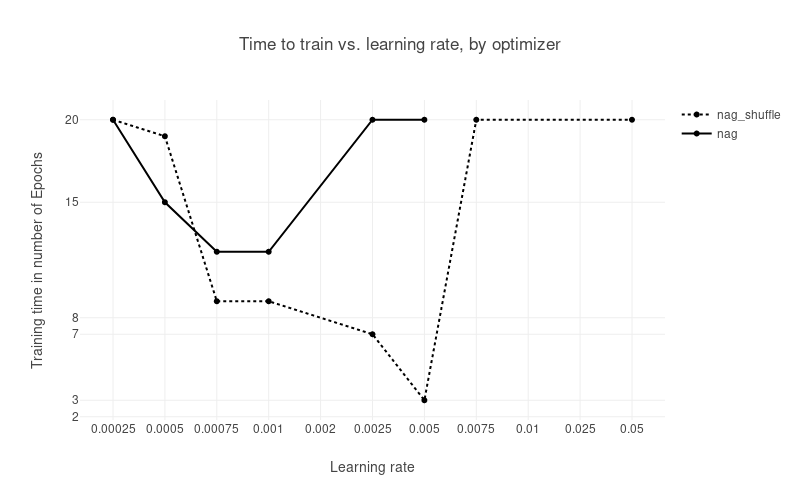
\includegraphics[scale=0.3]{images/results_nag_shuffle}
\caption{Training time Nesterov with input Shuffling}
\label{fig:results_nag}
\end{figure}
\subsubsection{Adagrad}
Adagrad \cite{adagrad} is a very interesting tool for learning word embeddings as it decreases the learning rate for very frequent occurring features, and vice versa). Because words that appear very frequently often do not have a semantic gain that is as important as words that appear less frequently to their context words, it's good to have a lower learning rate for such frequent words. So, in theory, Adagrad is particularly well suited for our task, as for example Pennington et al. used Adagrad in the training of Glove \cite{glove}, another system used to create word embeddings.  This was confirmed empirically as our model converged in 4 epochs. When combined with shuffling Adagrad only took 3 epochs to converge. This shows the tendency of the skip gram model to converge faster with input shuffling and the big impact of having different learning rate for each feature.
Here it's interesting to notice that a higher learning rate combined with input shuffling did not yield better results than without shuffling. Both of our best results happened with a learning rate of $0.1$, as shown in Figure \ref{fig:results_adagrad_shuffle}.
\begin{figure}[h]
\centering
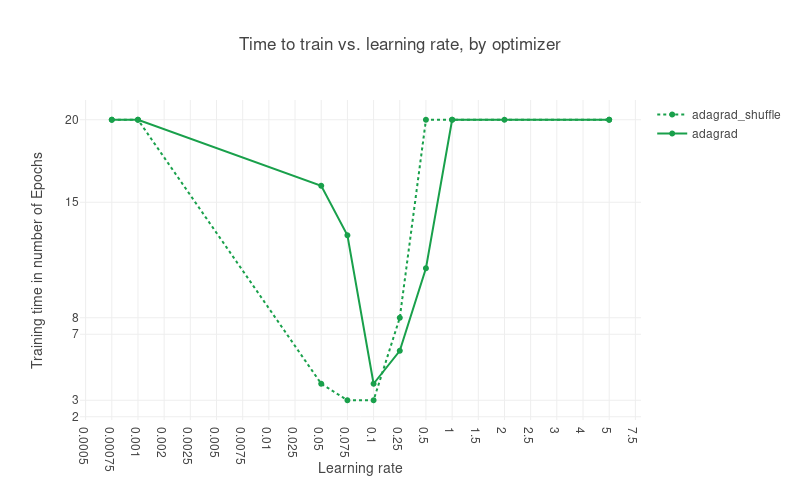
\includegraphics[scale=0.3]{images/results_adagrad_shuffle}
\caption{Training time Adagrad with input Shuffling}
\label{fig:results_adagrad_shuffle}
\end{figure}
\subsubsection{Adadelta}
In theory Adadelta \cite{adadelta} should outperform Adagrad as it's an extension of the former. Because it didn't have any learning rate to tune, we only did 2 experiments, with and without input shuffling. 
We are aware of the fact that there are additional hyper parameters to Adadelta. We decide not to tune theim for to reasons: first for simplicity reasons and second because their effect is not as high as the learning rate. The parameter that defines the percentage taken when calculating the exponentially decaying average of past gradients was set to $\rho = 0.9$. Adadelta did not manage to achieve a word similarity of 0.66. It only converged to a similarity of 0.59. It did this in 20 epochs without input shuffling and in 3 with input shuffling, as can be seen in Table \ref{table:results_adadelta}


\begin{table}[tb]
    \caption{Convergence Time and Quality with Adadelta}
    %\scriptsize
    \begin{tabular}{l r r }%
        \toprule
Adadelta Model & Convergence Time & Word similarity \\ 
        \midrule%
        Without Shuffling & 20 & 0.59 \\ 
With Shuffling & 3 & 0.59 \\
        \midrule%
   \end{tabular}%
   \label{table:results_adadelta}%
\end{table}

\subsubsection{Adam}
Adam is the most advanced of all the optimizers used in our experiments and did yield the best results as seen in Figure \ref{fig:results_adam_shuffle}. Adam converged in 3 epochs without shuffling and 2 with. This is the best result that we got with any optimizer.  It's also interesting to note that as same as with Adagrad it did not react to input shuffling the same way as SGD did. In fact, it worked in the opposite direction, as we achieved our best result with input shuffling while having a lower learning rate $0.001$ then we used to achieve the best result without input shuffling $0.05$.
\begin{figure}[h]
    \centering
            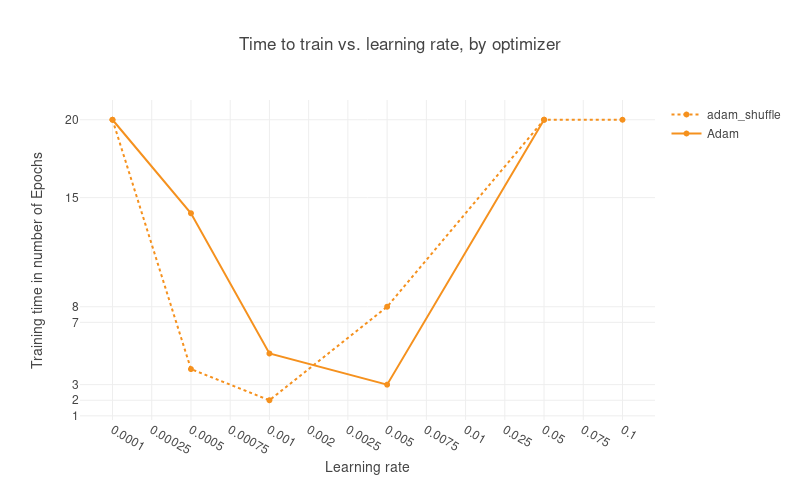
\includegraphics[scale=0.3]{images/results_adam_shuffle} 
    \caption{Training time Adam with input Shuffling}
    \label{fig:results_adam_shuffle}
\end{figure}